% Document Class is specified here. We're using the Homework Template
\documentclass[12pt, a4paper]{article}

\usepackage{graphicx}
\usepackage{float}
\usepackage{geometry}
\usepackage{verbatim}
\usepackage{listings}

\lstset{
  basicstyle=\itshape,
  xleftmargin=3em,
  literate={->}{$\rightarrow$}{2}
           {ε}{$\epsilon$}{1}
}

\geometry{a4paper, margin=1in}

\title{Week 9 CS-312 Homework}
\author{
	Cory Ness
	\and
	Jack Engledow
	\and
	James Sgrazzutti
}

\begin{document}

\maketitle

\section{Problem 11.5}
\subsection{Question}
Draw the diagram for a TM that accepts $\{0^{a}1^{b}: a < b\}$.
\subsection{Answer}
\begin{center}
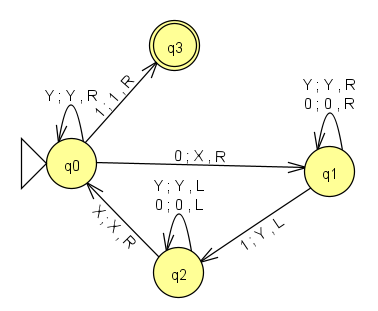
\includegraphics[scale=1]{11.5}
\end{center}

\section{Problem 11.7}
\subsection{Question}
Draw the diagram for a TM that accepts $\{a^{2^{n}}: n > 0\}$.
\subsection{Answer}
\begin{center}
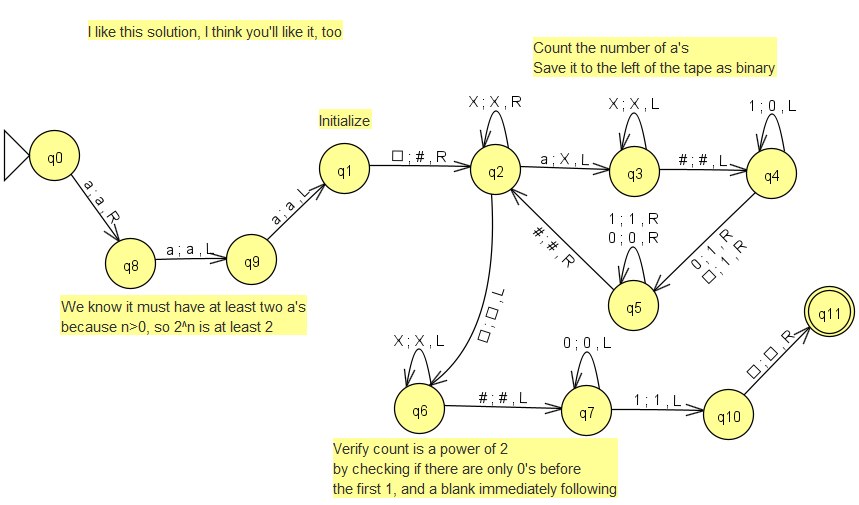
\includegraphics[scale=0.8]{11.7}
\end{center}

\section{Problem 11.17}
\subsection{Question}
Describe a TM subroutine that effectively deletes a symbol; that is, it deletes the symbol and shifts left all symbols to the right of this point.
\subsection{Answer}
The subroutine is defined as entering at the location of the symbol to delete, and follows the general format below, where there is a branch for every possible character of the tape alphabet.
\begin{center}
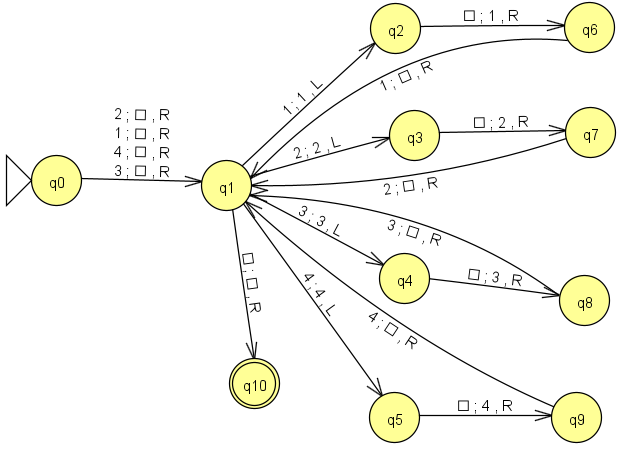
\includegraphics[scale=1]{11.17}
\end{center}

\section{Problem 12.3c}
\subsection{Question}
Write a TM that treat the input as a unary number and computes the remainder when the input is divided by 3.
\subsection{Answer}
Assuming that computed number is to be placed at the end of the unary number and that the symbol "a" will represent the unary symbol...
\begin{center}
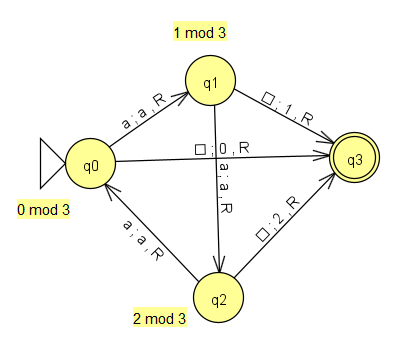
\includegraphics[scale=1]{12.3c}
\end{center}

\section{Problem 12.15}
\subsection{Question}
Suppose you have a TM $M$ for language $L$. Describe in English how to build a nondeterministic TM for language $L^{*}$.
\subsection{Answer}

\section{Problem 12.19}
\subsection{Question}
Sometimes a TM is defined to have a one-way infinite tape. The input is written at the start of the tape. The machine crashes if it tries to move off the left end of the tape.\newline
Sketch how to convert a program that runs on the standard TM model to that model, and vice versa.
\subsection{Answer}

\section{Problem 13.1}
\subsection{Question}
Let $M$ be an FA and $q$ some state of $M$. Call $q$ a useful state if there exists some input $w$ such that $M$ actually enters $q$. Let $B = \{<M,q>:q$ is a useful state of $M \}$. Show that $B$ is recursive.
\subsection{Answer}

\section{Problem 13.14}
\subsection{Question}
Show that if $L$ is accepted by a nondeterministic TM that always halts, then $L$ is recursive.
\subsection{Answer}

\section{Problem 13.18}
\subsection{Question}
Let language $Right_{tm} = \{M,w>: M$ is a TM that when started on input $w$ never moves its head left $\}$.
\subsubsection{Compute a quantity $Q$ such that, if $M$ runs for longer than this time on $w$ without moving its head left, then it will run forever.}
\subsubsection{Use this to show that $Right_{tm}$ is recursive.}


\end{document}